\documentclass{article}
\usepackage{nips_2016}

\usepackage[utf8]{inputenc} % allow utf-8 input
\usepackage[T1]{fontenc}    % use 8-bit T1 fonts
\usepackage{hyperref}       % hyperlinks
\usepackage{url}            % simple URL typesetting
\usepackage{booktabs}       % professional-quality tables
\usepackage{amsfonts}       % blackboard math symbols
\usepackage{nicefrac}       % compact symbols for 1/2, etc.
\usepackage{microtype}      % microtypography

\usepackage{graphicx}
\usepackage{tikz}
\usepackage{amssymb,amsmath}
%\usepackage{natbib}
\DeclareMathOperator*{\argmin}{arg\,min}
\DeclareMathOperator*{\sign}{sign}
\DeclareMathOperator*{\Lik}{Lik}
\DeclareMathOperator*{\Peaks}{Peaks}
\DeclareMathOperator*{\HotSpots}{HotSpots}
\newcommand{\Cost}{\text{Cost}}
\usepackage{stfloats}
\DeclareMathOperator*{\Diag}{Diag}
\DeclareMathOperator*{\TPR}{TPR}
\DeclareMathOperator*{\Segments}{Segments}
\DeclareMathOperator*{\Changes}{Changes}
\DeclareMathOperator*{\FPR}{FPR}
\DeclareMathOperator*{\argmax}{arg\,max}
\DeclareMathOperator*{\maximize}{maximize}
\DeclareMathOperator*{\minimize}{minimize}
\newcommand{\ZZ}{\mathbb Z}
\newcommand{\NN}{\mathbb N}
\newcommand{\RR}{\mathbb R}

\begin{document}

\title{A linear time algorithm for peak detection using constrained
  optimal segmentation}

\author{
  Toby Dylan Hocking\\
  Department of Human Genetics\\
  McGill University\\
  Montreal, QC H2R-2G9 Canada \\
  \texttt{toby.hocking@mail.mcgill.ca} \\
  %% examples of more authors
  \And
  Guillem Rigaill \\
  University of Evry \\
  Evry, France \\
  \texttt{guillem.rigaill@evry.fr} \\
  %% \AND
  %% Coauthor \\
  %% Affiliation \\
  %% Address \\
  %% \texttt{email} \\
  %% \And
  %% Coauthor \\
  %% Affiliation \\
  %% Address \\
  %% \texttt{email} \\
  %% \And
  %% Coauthor \\
  %% Affiliation \\
  %% Address \\
  %% \texttt{email} \\
}

\maketitle

\begin{abstract}
  Change-point detection is a central problem in time series and
  genomic data sets. We consider the PeakSeg constrained optimal
  segmentation model, for which the only previous solver is heuristic
  and quadratic time complexity. We propose a new Pruned Dynamic
  Programming Algorithm (PDPA) which recovers the exact solution in
  linear time. 
\end{abstract}

\section{Introduction}

\subsection{Peak detection in ChIP-seq data}

Chromatin immunoprecipitation sequencing (ChIP-seq) is a biological
experiment for genome-wide profiling of histone modifications and
transcription factor binding sites, with many experimental and
computational steps \citep{practical}. Briefly, each experiment yields
a set of sequence reads which are aligned to a reference genome, and
then the number of aligned reads are counted at each genomic position
(Figure~\ref{fig:good-bad}). Although these read counts can be
interpreted as quantitative data, they are most often interpreted
using one of the many available peak detection algorithms
\citep{evaluation2010, rye2010manually, chip-seq-bench}. A peak
detection algorithm is a binary classifier for each genomic
position. The positive class is enriched (peaks) and the negative
class is background noise. Importantly, peaks and background occur in
long contiguous segments across the genome.

More concretely, a single ChIP-seq profile on a genomic region with
$d$ base pairs can be represented as a vector $\mathbf y= \left[
  \begin{array}{ccc}
    y_1 & \cdots & y_d
  \end{array}
\right]\in\ZZ_+^d$ of counts of aligned sequence reads. A peak
detection algorithm is a function $c:\ZZ_+^d
\rightarrow \{0, 1\}^d$ which returns 0 for background noise and 1 for
a peak. 

\citet{pruned-dp} proposed a Pruned Dynamic Programming Algorithm
(PDPA) to exactly solve the penalized segmentation problem. In this
paper we use the FPOP algorithm to solve the penalized version of the
PeakSeg problem \citep{PeakSeg}.

\subsection{Contributions 
%and organization
}

The main contribution of this paper is a new Constrained Pruned
Dynamic Programming Algorithm (cPDPA) which is guaranteed to solve the
PeakSeg optimal segmentation problem. a peak detection model that can
be trained using supervised learning, and is effective for several
pattern types (sharp and broad peaks). Rather than taking unsupervised
model parameters for granted, we propose to train model parameters
using labeled data of the same pattern type. Importantly, and in
contrast to existing unsupervised approaches which can only be trained
using grid search, we propose efficient discrete and convex
optimization algorithms for model training. Our method is the first
peak detector with an efficient supervised learning algorithm, and the
first method that achieves state-of-the-art peak detection across
several patterns in the benchmark of \citet{hocking2014visual}.

A second contribution of this paper is a detailed study of the peak
detection accuracy of several unsupervised and supervised penalty
function learning methods. The two main results are that the oracle
penalty of \citet{cleynen2013segmentation} is more accurate than
asymptotic penalties like the AIC/BIC, and that supervised penalty
learning can be used to further increase peak detection accuracy.

\section{Related work}
\label{sec:related}

Our work is based on and inspired by roughly three types of related
work:
%Previous work can be divided into roughly three categories:
unsupervised ChIP-seq peak detectors from the bioinformatics
literature, maximum likelihood segmentation models, 
and criteria for model selection.

\subsection{Unsupervised ChIP-seq peak detectors}

There are literally dozens of unsupervised algorithms for peak
detection in ChIP-seq data sets, and the bioinformatics literature
contains several published comparison studies \citep{evaluation2010,
  rye2010manually, chip-seq-bench}. \citet{hocking2014visual} proposed
a benchmark of labeled ChIP-seq data sets, with two different histone
mark types: H3K4me3 (sharp peak pattern) and H3K36me3 (broad peak
pattern). The best peak detection algorithm in these H3K4me3 data was
macs \citep{MACS}, and the best for H3K36me3 was HMCan
\citep{HMCan}. Both of these algorithms are unsupervised, but were
calibrated via grid search using the annotated region labels to choose
the best scalar significance threshold hyperparameter.  Others have
proposed to train the hyperparameters of unsupervised peak detectors
\citep{picking2012, DFilter}. In contrast, we propose the supervised
\ref{PeakSeg} model which can be efficiently trained using discrete
and convex optimization algorithms (Sections~\ref{sec:algorithms} and
\ref{sec:penalty-learning}).

\subsection{Maximum likelihood segmentation models}

The \ref{PeakSeg} model we propose in this paper is a constrained
version of the Poisson segmentation model of \citet{Segmentor}.
Their unconstrained model can be computed using a dynamic programming
algorithm (DPA) \citep{bellman}, or a pruned dynamic programming
algorithm (pDPA) \citep{pruned-dp}. Both algorithms are guaranteed to
recover the exact solution to the unconstrained model, but there are
two important differences. The pDPA is more complicated to implement,
but is also computationally faster than the DPA. For segmenting a
sequence of $d$ data points, the pDPA takes on average $O(d\log d)$
time whereas the DPA takes $O(d^2)$ time. 

Relative to the unconstrained segmentation model of \citet{Segmentor},
our proposed \ref{PeakSeg} model has an additional constraint. Rather
than searching all possible change-points to find the most likely
model with $s$ segments, we propose to constrain the possible
change-points to the subset of models that can be interpreted as peaks
(with segment means that change up, down, up, etc, see
Section~\ref{sec:constrained}).

Due to the simplicity of its implementation, we propose a constrained
dynamic programming algorithm (cDPA) that requires a small
modification to the standard DPA solver. Although the DPA is an exact
solver for the unconstrained problem, we show that the cDPA is a
heuristic that is not guaranteed to solve the constrained
problem (Section~\ref{sec:dp-fails}). However, we show that it is
still very useful and accurate in practice on real data
(Section~\ref{sec:results}).


\section{Problem setting}

\subsection{Unconstrained model}

We have a genomic data set $\mathbf{z}\in\ZZ_+^B$ of counts on $B$
bases. The unconstrained problem for a positive penalty parameter
$\lambda\in\RR_+$ is
\begin{equation}
  \label{unconstrained}
  \mathbf{\hat m}^\lambda(\mathbf z)  =\ 
  \argmin_{\mathbf m\in\RR^{B}}\ 
  \rho
  %\tag{\textbf{Unconstrained}}
  (\mathbf m, \mathbf z) 
  +\lambda\Changes(\mathbf m),
\end{equation}
where the Poisson loss function is
\begin{equation}\label{eq:rho}
  \rho(\mathbf m, \mathbf z)= \sum_{b=1}^B m_b - z_b \log m_b.
\end{equation} 
The model complexity is the number of change-points
\begin{equation}
  \Changes(\mathbf m)=\sum_{b=2}^B I(m_{b-1} \neq m_b),
\end{equation}
where $I$ is the indicator function.

Although it is a non-convex optimization problem, the segmentation
$\mathbf{\hat m}^\lambda(\mathbf z)$ can be computed in linear $O(B)$
time using the FPOP algorithm \citep{FPOP}.

We refer to (\ref{unconstrained}) as the ``unconstrained'' model since
$\mathbf{\hat m}^\lambda(\mathbf z)$ can have any sequence of changes
up or down. However for the purposes of peak detection, we are only
interested in segmentations with alternating changes that can be
interpreted as peaks and background \citep{PeakSeg}.

More concretely, we first define the peak indicator at base
$b\in\{2, \dots, B\}$ as
\begin{equation}
  \label{eq:peaks}
  P_b(\mathbf m) = \sum_{j=2}^b \sign( m_{j} - m_{j-1} ),
\end{equation}
where $P_1(\mathbf m)=0$ by convention. $P_b(\mathbf m)$ is the
cumulative sum of signs of changes up to point $b$ in the piecewise
constant vector $\mathbf m$. We define the vector of peak indicators
as
\begin{equation}
  \mathbf
  P[\mathbf m] = \left[
    \begin{array}{ccc}
      P_1(\mathbf m) & \cdots & P_B(\mathbf m)
    \end{array}\right].
\end{equation}

\subsection{PenPeakSeg: penalized constrained segmentation}
\label{sec:constrained}

In general for the unconstrained model $P_b(\mathbf m)\in\ZZ$, which
is problematic since we want to use it as a peak detector with binary
outputs $P_b(\mathbf m)\in \{0, 1\}$. 
For example, if $\mathbf m = \left[\begin{array}{ccccccc}1.1 &
    1.1 & 2 & 2 & 4 & 4 & 3\end{array}\right]$, with two changes up
followed by one change down, then $\mathbf P(\mathbf m) =
\left[\begin{array}{ccccccc}0 & 0 & 1 & 1 & 2 & 2 &
    1 \end{array}\right]$.
Thus we constrain the peak indicator $P_b(\mathbf m)\in\{0, 1\}$,
which results in the constrained problem
\begin{align*}
  \label{PenPeakSeg}
  \mathbf{\tilde m}^\lambda(\mathbf z)  =
  \argmin_{\mathbf m\in\RR^{B}} &\ \ 
    \rho(\mathbf m, \mathbf z) + \lambda\Peaks(\mathbf m)
    \tag{\textbf{PenPeakSeg}}
  \\
  \text{such that} &\ \forall b\in\{1, \dots, B\},
                     \ \ P_b(\mathbf m) \in\{0, 1\}.
\end{align*}
The Peaks model complexity term only counts up changes:
\begin{equation}
  \Peaks(\mathbf m) = \sum_{b=2}^B I(m_{b-1} < m_b).
\end{equation}
The constraint in the \ref{PenPeakSeg} problem forces the sequence of
changes in the segment means $\mathbf m$ to begin with a positive
change and then alternate: up, down, up, down, ... (and not up, up,
down). Thus the even-numbered segments may be interpreted as peaks
$P_b(\mathbf m)=1$, and the odd-numbered segments may be interpreted
as background $P_b(\mathbf m)=0$.

\section{Algorithm}

\subsection{Segment Neighborhood}

For the Segment Neighborhood algorithm we begin as usual by computing
a functional representation of the optimal cost in 1 segment up to
base $b$. 
\begin{equation*}
  \label{eq:C1b}
  C_{1,b}(\mu) = \sum_{i=1}^b \gamma_b(\mu),
\end{equation*}
where $\gamma_b(\mu)$ is the cost of using the mean $\mu$ for single
data point $b$ (for example the Gaussian or Poisson loss).

Next we define the minimum cost in 2 segments up to data point 2 as
\begin{equation*}
  \label{eq:C22}
  C_{2,2}(\mu) = C_{1,1}^{\leq}(\mu) + \gamma_2(\mu),
\end{equation*}
where for a function $f:\RR\rightarrow\RR$ the min-less operator
yields another function $f\leq:\RR\rightarrow\RR$ such that
\begin{equation}
  \label{eq:min-less}
  f^{\leq}(\mu) = \min_{x\leq \mu} f(x).
\end{equation}
The algorithm relies on the ability to compute an exact representation
of functions such as $C_{1,1}^{\leq}$. Since the cost functions $f$
are quasiconvex, we can easily find the minimum $\mu^*$, and then
compute the following exact representation
\begin{equation*}
  f^\leq(\mu)
  \begin{cases}
    f(\mu^*) & \text{ if } \mu \geq \mu^*,\\
    f(\mu) & \text{ otherwise.}
  \end{cases}
\end{equation*}

\begin{figure}[!t]
  \parbox{3in}{
    \begin{center}
    % Created by tikzDevice version 0.7.0 on 2016-06-06 10:57:28
% !TEX encoding = UTF-8 Unicode
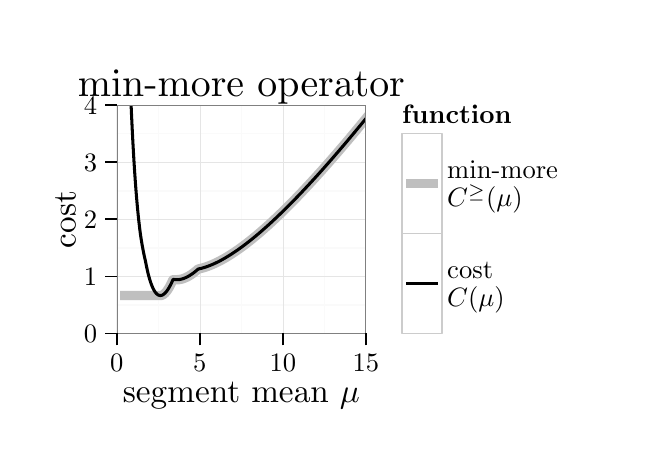
\begin{tikzpicture}[x=1pt,y=1pt]
\definecolor[named]{fillColor}{rgb}{1.00,1.00,1.00}
\path[use as bounding box,fill=fillColor,fill opacity=0.00] (0,0) rectangle (216.81,144.54);
\begin{scope}
\path[clip] (  0.00,  0.00) rectangle (216.81,144.54);
\definecolor[named]{drawColor}{rgb}{1.00,1.00,1.00}
\definecolor[named]{fillColor}{rgb}{1.00,1.00,1.00}

\path[draw=drawColor,line width= 0.6pt,line join=round,line cap=round,fill=fillColor] (  0.00,  0.00) rectangle (216.81,144.54);
\end{scope}
\begin{scope}
\path[clip] ( 32.22, 34.03) rectangle (122.22,116.55);
\definecolor[named]{fillColor}{rgb}{1.00,1.00,1.00}

\path[fill=fillColor] ( 32.22, 34.03) rectangle (122.22,116.55);
\definecolor[named]{drawColor}{rgb}{0.98,0.98,0.98}

\path[draw=drawColor,line width= 0.6pt,line join=round] ( 32.22, 44.35) --
	(122.22, 44.35);

\path[draw=drawColor,line width= 0.6pt,line join=round] ( 32.22, 64.98) --
	(122.22, 64.98);

\path[draw=drawColor,line width= 0.6pt,line join=round] ( 32.22, 85.61) --
	(122.22, 85.61);

\path[draw=drawColor,line width= 0.6pt,line join=round] ( 32.22,106.24) --
	(122.22,106.24);

\path[draw=drawColor,line width= 0.6pt,line join=round] ( 47.22, 34.03) --
	( 47.22,116.55);

\path[draw=drawColor,line width= 0.6pt,line join=round] ( 77.22, 34.03) --
	( 77.22,116.55);

\path[draw=drawColor,line width= 0.6pt,line join=round] (107.22, 34.03) --
	(107.22,116.55);
\definecolor[named]{drawColor}{rgb}{0.90,0.90,0.90}

\path[draw=drawColor,line width= 0.2pt,line join=round] ( 32.22, 34.03) --
	(122.22, 34.03);

\path[draw=drawColor,line width= 0.2pt,line join=round] ( 32.22, 54.66) --
	(122.22, 54.66);

\path[draw=drawColor,line width= 0.2pt,line join=round] ( 32.22, 75.29) --
	(122.22, 75.29);

\path[draw=drawColor,line width= 0.2pt,line join=round] ( 32.22, 95.92) --
	(122.22, 95.92);

\path[draw=drawColor,line width= 0.2pt,line join=round] ( 32.22,116.55) --
	(122.22,116.55);

\path[draw=drawColor,line width= 0.2pt,line join=round] ( 32.22, 34.03) --
	( 32.22,116.55);

\path[draw=drawColor,line width= 0.2pt,line join=round] ( 62.22, 34.03) --
	( 62.22,116.55);

\path[draw=drawColor,line width= 0.2pt,line join=round] ( 92.22, 34.03) --
	( 92.22,116.55);

\path[draw=drawColor,line width= 0.2pt,line join=round] (122.22, 34.03) --
	(122.22,116.55);
\definecolor[named]{drawColor}{rgb}{0.75,0.75,0.75}

\path[draw=drawColor,line width= 3.4pt,line join=round] ( 33.40, 47.76) --
	( 33.55, 47.76) --
	( 33.70, 47.76) --
	( 33.84, 47.76) --
	( 33.99, 47.76) --
	( 34.14, 47.76) --
	( 34.28, 47.76) --
	( 34.43, 47.76) --
	( 34.58, 47.76) --
	( 34.73, 47.76) --
	( 34.87, 47.76) --
	( 35.02, 47.76) --
	( 35.17, 47.76) --
	( 35.31, 47.76) --
	( 35.46, 47.76) --
	( 35.61, 47.76) --
	( 35.75, 47.76) --
	( 35.90, 47.76) --
	( 36.05, 47.76) --
	( 36.19, 47.76) --
	( 36.34, 47.76) --
	( 36.49, 47.76) --
	( 36.63, 47.76) --
	( 36.78, 47.76) --
	( 36.93, 47.76) --
	( 37.08, 47.76) --
	( 37.22, 47.76) --
	( 37.37, 47.76) --
	( 37.52, 47.76) --
	( 37.66, 47.76) --
	( 37.81, 47.76) --
	( 37.96, 47.76) --
	( 38.10, 47.76) --
	( 38.25, 47.76) --
	( 38.40, 47.76) --
	( 38.54, 47.76) --
	( 38.69, 47.76) --
	( 38.84, 47.76) --
	( 38.98, 47.76) --
	( 39.13, 47.76) --
	( 39.28, 47.76) --
	( 39.43, 47.76) --
	( 39.57, 47.76) --
	( 39.72, 47.76) --
	( 39.87, 47.76) --
	( 40.01, 47.76) --
	( 40.16, 47.76) --
	( 40.31, 47.76) --
	( 40.45, 47.76) --
	( 40.60, 47.76) --
	( 40.75, 47.76) --
	( 40.89, 47.76) --
	( 41.04, 47.76) --
	( 41.19, 47.76) --
	( 41.34, 47.76) --
	( 41.48, 47.76) --
	( 41.63, 47.76) --
	( 41.78, 47.76) --
	( 41.92, 47.76) --
	( 42.07, 47.76) --
	( 42.22, 47.76) --
	( 42.36, 47.76) --
	( 42.51, 47.76) --
	( 42.66, 47.76) --
	( 42.80, 47.76) --
	( 42.95, 47.76) --
	( 43.10, 47.76) --
	( 43.24, 47.76) --
	( 43.39, 47.76) --
	( 43.54, 47.76) --
	( 43.69, 47.76) --
	( 43.83, 47.76) --
	( 43.98, 47.76) --
	( 44.13, 47.76) --
	( 44.27, 47.76) --
	( 44.42, 47.76) --
	( 44.57, 47.76) --
	( 44.71, 47.76) --
	( 44.86, 47.76) --
	( 45.01, 47.76) --
	( 45.15, 47.76) --
	( 45.30, 47.76) --
	( 45.45, 47.76) --
	( 45.59, 47.76) --
	( 45.74, 47.76) --
	( 45.89, 47.76) --
	( 46.04, 47.76) --
	( 46.18, 47.76) --
	( 46.33, 47.76) --
	( 46.48, 47.76) --
	( 46.62, 47.76) --
	( 46.77, 47.76) --
	( 46.92, 47.76) --
	( 47.06, 47.76) --
	( 47.21, 47.76) --
	( 47.36, 47.76) --
	( 47.50, 47.76) --
	( 47.65, 47.76) --
	( 47.80, 47.76) --
	( 47.94, 47.76) --
	( 47.94, 47.76) --
	( 47.99, 47.76) --
	( 48.04, 47.76) --
	( 48.08, 47.76) --
	( 48.13, 47.77) --
	( 48.17, 47.77) --
	( 48.22, 47.78) --
	( 48.27, 47.79) --
	( 48.31, 47.80) --
	( 48.36, 47.81) --
	( 48.40, 47.82) --
	( 48.45, 47.84) --
	( 48.50, 47.85) --
	( 48.54, 47.87) --
	( 48.59, 47.89) --
	( 48.63, 47.91) --
	( 48.68, 47.93) --
	( 48.73, 47.95) --
	( 48.77, 47.97) --
	( 48.82, 48.00) --
	( 48.86, 48.02) --
	( 48.91, 48.05) --
	( 48.95, 48.08) --
	( 49.00, 48.11) --
	( 49.05, 48.14) --
	( 49.09, 48.17) --
	( 49.14, 48.20) --
	( 49.18, 48.24) --
	( 49.23, 48.27) --
	( 49.28, 48.31) --
	( 49.32, 48.35) --
	( 49.37, 48.38) --
	( 49.41, 48.42) --
	( 49.46, 48.47) --
	( 49.51, 48.51) --
	( 49.55, 48.55) --
	( 49.60, 48.60) --
	( 49.64, 48.64) --
	( 49.69, 48.69) --
	( 49.74, 48.74) --
	( 49.78, 48.78) --
	( 49.83, 48.83) --
	( 49.87, 48.89) --
	( 49.92, 48.94) --
	( 49.97, 48.99) --
	( 50.01, 49.05) --
	( 50.06, 49.10) --
	( 50.10, 49.16) --
	( 50.15, 49.22) --
	( 50.19, 49.27) --
	( 50.24, 49.33) --
	( 50.29, 49.40) --
	( 50.33, 49.46) --
	( 50.38, 49.52) --
	( 50.42, 49.58) --
	( 50.47, 49.65) --
	( 50.52, 49.72) --
	( 50.56, 49.78) --
	( 50.61, 49.85) --
	( 50.65, 49.92) --
	( 50.70, 49.99) --
	( 50.75, 50.06) --
	( 50.79, 50.13) --
	( 50.84, 50.21) --
	( 50.88, 50.28) --
	( 50.93, 50.36) --
	( 50.98, 50.43) --
	( 51.02, 50.51) --
	( 51.07, 50.59) --
	( 51.11, 50.67) --
	( 51.16, 50.75) --
	( 51.21, 50.83) --
	( 51.25, 50.91) --
	( 51.30, 50.99) --
	( 51.34, 51.07) --
	( 51.39, 51.16) --
	( 51.43, 51.25) --
	( 51.48, 51.33) --
	( 51.53, 51.42) --
	( 51.57, 51.51) --
	( 51.62, 51.60) --
	( 51.66, 51.69) --
	( 51.71, 51.78) --
	( 51.76, 51.87) --
	( 51.80, 51.96) --
	( 51.85, 52.06) --
	( 51.89, 52.15) --
	( 51.94, 52.25) --
	( 51.99, 52.34) --
	( 52.03, 52.44) --
	( 52.08, 52.54) --
	( 52.12, 52.64) --
	( 52.17, 52.74) --
	( 52.22, 52.84) --
	( 52.26, 52.94) --
	( 52.31, 53.04) --
	( 52.35, 53.15) --
	( 52.40, 53.25) --
	( 52.45, 53.35) --
	( 52.49, 53.46) --
	( 52.49, 53.46) --
	( 52.50, 53.46) --
	( 52.52, 53.46) --
	( 52.53, 53.46) --
	( 52.55, 53.46) --
	( 52.56, 53.46) --
	( 52.57, 53.46) --
	( 52.59, 53.46) --
	( 52.60, 53.46) --
	( 52.62, 53.46) --
	( 52.63, 53.46) --
	( 52.64, 53.46) --
	( 52.66, 53.46) --
	( 52.67, 53.46) --
	( 52.68, 53.46) --
	( 52.70, 53.46) --
	( 52.71, 53.46) --
	( 52.73, 53.46) --
	( 52.74, 53.46) --
	( 52.75, 53.46) --
	( 52.77, 53.46) --
	( 52.78, 53.46) --
	( 52.80, 53.46) --
	( 52.81, 53.46) --
	( 52.82, 53.46) --
	( 52.84, 53.46) --
	( 52.85, 53.46) --
	( 52.86, 53.46) --
	( 52.88, 53.46) --
	( 52.89, 53.46) --
	( 52.91, 53.46) --
	( 52.92, 53.46) --
	( 52.93, 53.46) --
	( 52.95, 53.46) --
	( 52.96, 53.46) --
	( 52.97, 53.46) --
	( 52.99, 53.46) --
	( 53.00, 53.46) --
	( 53.02, 53.46) --
	( 53.03, 53.46) --
	( 53.04, 53.46) --
	( 53.06, 53.46) --
	( 53.07, 53.46) --
	( 53.09, 53.46) --
	( 53.10, 53.46) --
	( 53.11, 53.46) --
	( 53.13, 53.46) --
	( 53.14, 53.46) --
	( 53.15, 53.46) --
	( 53.17, 53.46) --
	( 53.18, 53.46) --
	( 53.20, 53.46) --
	( 53.21, 53.46) --
	( 53.22, 53.46) --
	( 53.24, 53.46) --
	( 53.25, 53.46) --
	( 53.26, 53.46) --
	( 53.28, 53.46) --
	( 53.29, 53.46) --
	( 53.31, 53.46) --
	( 53.32, 53.46) --
	( 53.33, 53.46) --
	( 53.35, 53.46) --
	( 53.36, 53.46) --
	( 53.38, 53.46) --
	( 53.39, 53.46) --
	( 53.40, 53.46) --
	( 53.42, 53.46) --
	( 53.43, 53.46) --
	( 53.44, 53.46) --
	( 53.46, 53.46) --
	( 53.47, 53.46) --
	( 53.49, 53.46) --
	( 53.50, 53.46) --
	( 53.51, 53.46) --
	( 53.53, 53.46) --
	( 53.54, 53.46) --
	( 53.56, 53.46) --
	( 53.57, 53.46) --
	( 53.58, 53.46) --
	( 53.60, 53.46) --
	( 53.61, 53.46) --
	( 53.62, 53.46) --
	( 53.64, 53.46) --
	( 53.65, 53.46) --
	( 53.67, 53.46) --
	( 53.68, 53.46) --
	( 53.69, 53.46) --
	( 53.71, 53.46) --
	( 53.72, 53.46) --
	( 53.73, 53.46) --
	( 53.75, 53.46) --
	( 53.76, 53.46) --
	( 53.78, 53.46) --
	( 53.79, 53.46) --
	( 53.80, 53.46) --
	( 53.82, 53.46) --
	( 53.83, 53.46) --
	( 53.85, 53.46) --
	( 53.86, 53.46) --
	( 53.86, 53.46) --
	( 53.94, 53.46) --
	( 54.02, 53.46) --
	( 54.09, 53.47) --
	( 54.17, 53.47) --
	( 54.25, 53.47) --
	( 54.33, 53.48) --
	( 54.41, 53.48) --
	( 54.48, 53.49) --
	( 54.56, 53.50) --
	( 54.64, 53.51) --
	( 54.72, 53.52) --
	( 54.80, 53.53) --
	( 54.87, 53.54) --
	( 54.95, 53.55) --
	( 55.03, 53.57) --
	( 55.11, 53.58) --
	( 55.19, 53.60) --
	( 55.26, 53.61) --
	( 55.34, 53.63) --
	( 55.42, 53.65) --
	( 55.50, 53.66) --
	( 55.58, 53.68) --
	( 55.65, 53.70) --
	( 55.73, 53.72) --
	( 55.81, 53.75) --
	( 55.89, 53.77) --
	( 55.97, 53.79) --
	( 56.04, 53.82) --
	( 56.12, 53.84) --
	( 56.20, 53.87) --
	( 56.28, 53.89) --
	( 56.36, 53.92) --
	( 56.43, 53.95) --
	( 56.51, 53.98) --
	( 56.59, 54.01) --
	( 56.67, 54.04) --
	( 56.75, 54.07) --
	( 56.82, 54.10) --
	( 56.90, 54.13) --
	( 56.98, 54.17) --
	( 57.06, 54.20) --
	( 57.14, 54.24) --
	( 57.21, 54.27) --
	( 57.29, 54.31) --
	( 57.37, 54.35) --
	( 57.45, 54.38) --
	( 57.53, 54.42) --
	( 57.60, 54.46) --
	( 57.68, 54.50) --
	( 57.76, 54.54) --
	( 57.84, 54.58) --
	( 57.92, 54.62) --
	( 57.99, 54.67) --
	( 58.07, 54.71) --
	( 58.15, 54.75) --
	( 58.23, 54.80) --
	( 58.31, 54.84) --
	( 58.38, 54.89) --
	( 58.46, 54.94) --
	( 58.54, 54.98) --
	( 58.62, 55.03) --
	( 58.70, 55.08) --
	( 58.77, 55.13) --
	( 58.85, 55.18) --
	( 58.93, 55.23) --
	( 59.01, 55.28) --
	( 59.09, 55.33) --
	( 59.16, 55.39) --
	( 59.24, 55.44) --
	( 59.32, 55.49) --
	( 59.40, 55.55) --
	( 59.48, 55.60) --
	( 59.55, 55.66) --
	( 59.63, 55.72) --
	( 59.71, 55.77) --
	( 59.79, 55.83) --
	( 59.87, 55.89) --
	( 59.94, 55.95) --
	( 60.02, 56.00) --
	( 60.10, 56.06) --
	( 60.18, 56.13) --
	( 60.26, 56.19) --
	( 60.33, 56.25) --
	( 60.41, 56.31) --
	( 60.49, 56.37) --
	( 60.57, 56.44) --
	( 60.65, 56.50) --
	( 60.72, 56.56) --
	( 60.80, 56.63) --
	( 60.88, 56.69) --
	( 60.96, 56.76) --
	( 61.04, 56.83) --
	( 61.11, 56.89) --
	( 61.19, 56.96) --
	( 61.27, 57.03) --
	( 61.35, 57.10) --
	( 61.43, 57.17) --
	( 61.50, 57.24) --
	( 61.58, 57.31) --
	( 61.58, 57.31) --
	( 62.58, 57.54) --
	( 63.58, 57.81) --
	( 64.59, 58.14) --
	( 65.59, 58.50) --
	( 66.59, 58.91) --
	( 67.59, 59.35) --
	( 68.59, 59.83) --
	( 69.60, 60.34) --
	( 70.60, 60.89) --
	( 71.60, 61.46) --
	( 72.60, 62.07) --
	( 73.60, 62.70) --
	( 74.60, 63.36) --
	( 75.61, 64.04) --
	( 76.61, 64.75) --
	( 77.61, 65.47) --
	( 78.61, 66.23) --
	( 79.61, 67.00) --
	( 80.62, 67.79) --
	( 81.62, 68.60) --
	( 82.62, 69.43) --
	( 83.62, 70.27) --
	( 84.62, 71.14) --
	( 85.62, 72.02) --
	( 86.63, 72.91) --
	( 87.63, 73.82) --
	( 88.63, 74.75) --
	( 89.63, 75.69) --
	( 90.63, 76.64) --
	( 91.63, 77.60) --
	( 92.64, 78.58) --
	( 93.64, 79.57) --
	( 94.64, 80.57) --
	( 95.64, 81.59) --
	( 96.64, 82.61) --
	( 97.65, 83.65) --
	( 98.65, 84.69) --
	( 99.65, 85.75) --
	(100.65, 86.82) --
	(101.65, 87.89) --
	(102.65, 88.98) --
	(103.66, 90.07) --
	(104.66, 91.17) --
	(105.66, 92.28) --
	(106.66, 93.40) --
	(107.66, 94.53) --
	(108.66, 95.66) --
	(109.67, 96.81) --
	(110.67, 97.96) --
	(111.67, 99.12) --
	(112.67,100.28) --
	(113.67,101.45) --
	(114.68,102.63) --
	(115.68,103.81) --
	(116.68,105.01) --
	(117.68,106.20) --
	(118.68,107.41) --
	(119.68,108.62) --
	(120.69,109.83) --
	(121.69,111.05) --
	(122.69,112.28) --
	(123.69,113.51) --
	(124.69,114.75) --
	(125.69,115.99) --
	(126.70,117.24) --
	(127.70,118.49) --
	(128.70,119.75) --
	(129.70,121.01) --
	(130.70,122.28) --
	(131.71,123.55) --
	(132.71,124.83) --
	(133.71,126.11) --
	(134.71,127.39) --
	(135.71,128.68) --
	(136.71,129.98) --
	(137.72,131.28) --
	(138.72,132.58) --
	(139.72,133.88) --
	(140.72,135.19) --
	(141.72,136.51) --
	(142.73,137.82) --
	(143.73,139.14) --
	(144.73,140.47) --
	(145.73,141.80) --
	(146.73,143.13) --
	(147.73,144.46) --
	(147.79,144.54);
\definecolor[named]{drawColor}{rgb}{0.00,0.00,0.00}

\path[draw=drawColor,line width= 1.1pt,line join=round] ( 36.37,144.54) --
	( 36.37,144.21) --
	( 36.45,141.63) --
	( 36.53,139.12) --
	( 36.61,136.68) --
	( 36.69,134.31) --
	( 36.77,132.01) --
	( 36.85,129.77) --
	( 36.93,127.59) --
	( 37.01,125.48) --
	( 37.09,123.42) --
	( 37.17,121.41) --
	( 37.25,119.46) --
	( 37.33,117.56) --
	( 37.41,115.72) --
	( 37.49,113.92) --
	( 37.57,112.17) --
	( 37.65,110.46) --
	( 37.73,108.80) --
	( 37.81,107.19) --
	( 37.89,105.61) --
	( 37.97,104.08) --
	( 38.05,102.59) --
	( 38.13,101.14) --
	( 38.21, 99.72) --
	( 38.29, 98.34) --
	( 38.37, 97.00) --
	( 38.45, 95.69) --
	( 38.53, 94.42) --
	( 38.61, 93.18) --
	( 38.69, 91.97) --
	( 38.77, 90.79) --
	( 38.85, 89.65) --
	( 38.93, 88.53) --
	( 39.01, 87.45) --
	( 39.09, 86.39) --
	( 39.17, 85.36) --
	( 39.25, 84.36) --
	( 39.33, 83.39) --
	( 39.41, 82.44) --
	( 39.49, 81.52) --
	( 39.57, 80.62) --
	( 39.65, 79.74) --
	( 39.73, 78.90) --
	( 39.81, 78.07) --
	( 39.89, 77.27) --
	( 39.97, 76.49) --
	( 40.05, 75.73) --
	( 40.13, 74.99) --
	( 40.21, 74.28) --
	( 40.29, 73.58) --
	( 40.37, 72.91) --
	( 40.44, 72.25) --
	( 40.52, 71.62) --
	( 40.60, 71.00) --
	( 40.68, 70.41) --
	( 40.76, 69.83) --
	( 40.84, 69.27) --
	( 40.92, 68.73) --
	( 41.00, 68.20) --
	( 41.08, 67.69) --
	( 41.16, 67.20) --
	( 41.24, 66.73) --
	( 41.32, 66.27) --
	( 41.40, 65.83) --
	( 41.48, 65.40) --
	( 41.56, 64.99) --
	( 41.56, 64.99) --
	( 41.57, 64.93) --
	( 41.58, 64.88) --
	( 41.59, 64.82) --
	( 41.60, 64.76) --
	( 41.61, 64.71) --
	( 41.62, 64.65) --
	( 41.63, 64.59) --
	( 41.64, 64.54) --
	( 41.65, 64.48) --
	( 41.66, 64.43) --
	( 41.67, 64.37) --
	( 41.68, 64.32) --
	( 41.69, 64.26) --
	( 41.70, 64.21) --
	( 41.71, 64.15) --
	( 41.72, 64.10) --
	( 41.73, 64.04) --
	( 41.74, 63.99) --
	( 41.75, 63.94) --
	( 41.76, 63.88) --
	( 41.77, 63.83) --
	( 41.78, 63.78) --
	( 41.79, 63.72) --
	( 41.80, 63.67) --
	( 41.81, 63.62) --
	( 41.82, 63.57) --
	( 41.83, 63.52) --
	( 41.84, 63.46) --
	( 41.85, 63.41) --
	( 41.86, 63.36) --
	( 41.87, 63.31) --
	( 41.88, 63.26) --
	( 41.89, 63.21) --
	( 41.90, 63.16) --
	( 41.91, 63.11) --
	( 41.92, 63.06) --
	( 41.93, 63.01) --
	( 41.94, 62.96) --
	( 41.95, 62.91) --
	( 41.96, 62.86) --
	( 41.97, 62.81) --
	( 41.98, 62.76) --
	( 41.99, 62.71) --
	( 42.00, 62.67) --
	( 42.01, 62.62) --
	( 42.02, 62.57) --
	( 42.03, 62.52) --
	( 42.04, 62.48) --
	( 42.05, 62.43) --
	( 42.06, 62.38) --
	( 42.07, 62.33) --
	( 42.08, 62.29) --
	( 42.09, 62.24) --
	( 42.10, 62.19) --
	( 42.11, 62.15) --
	( 42.12, 62.10) --
	( 42.13, 62.06) --
	( 42.14, 62.01) --
	( 42.15, 61.97) --
	( 42.16, 61.92) --
	( 42.17, 61.88) --
	( 42.18, 61.83) --
	( 42.19, 61.79) --
	( 42.20, 61.74) --
	( 42.21, 61.70) --
	( 42.22, 61.65) --
	( 42.22, 61.61) --
	( 42.23, 61.57) --
	( 42.24, 61.52) --
	( 42.25, 61.48) --
	( 42.26, 61.44) --
	( 42.27, 61.39) --
	( 42.28, 61.35) --
	( 42.29, 61.31) --
	( 42.30, 61.27) --
	( 42.31, 61.23) --
	( 42.32, 61.18) --
	( 42.33, 61.14) --
	( 42.34, 61.10) --
	( 42.35, 61.06) --
	( 42.36, 61.02) --
	( 42.37, 60.98) --
	( 42.38, 60.94) --
	( 42.39, 60.90) --
	( 42.40, 60.86) --
	( 42.41, 60.82) --
	( 42.42, 60.78) --
	( 42.43, 60.74) --
	( 42.44, 60.70) --
	( 42.45, 60.66) --
	( 42.46, 60.62) --
	( 42.47, 60.58) --
	( 42.48, 60.54) --
	( 42.49, 60.50) --
	( 42.50, 60.46) --
	( 42.51, 60.43) --
	( 42.52, 60.39) --
	( 42.53, 60.35) --
	( 42.54, 60.31) --
	( 42.54, 60.31) --
	( 42.64, 59.77) --
	( 42.74, 59.25) --
	( 42.84, 58.74) --
	( 42.95, 58.25) --
	( 43.05, 57.77) --
	( 43.15, 57.31) --
	( 43.25, 56.85) --
	( 43.35, 56.42) --
	( 43.45, 55.99) --
	( 43.55, 55.58) --
	( 43.65, 55.18) --
	( 43.75, 54.80) --
	( 43.86, 54.43) --
	( 43.96, 54.07) --
	( 44.06, 53.72) --
	( 44.16, 53.38) --
	( 44.26, 53.06) --
	( 44.36, 52.74) --
	( 44.46, 52.44) --
	( 44.56, 52.15) --
	( 44.66, 51.87) --
	( 44.77, 51.60) --
	( 44.87, 51.34) --
	( 44.97, 51.09) --
	( 45.07, 50.85) --
	( 45.17, 50.62) --
	( 45.27, 50.41) --
	( 45.37, 50.20) --
	( 45.47, 50.00) --
	( 45.57, 49.81) --
	( 45.68, 49.63) --
	( 45.78, 49.46) --
	( 45.88, 49.29) --
	( 45.98, 49.14) --
	( 46.08, 49.00) --
	( 46.18, 48.86) --
	( 46.28, 48.73) --
	( 46.38, 48.61) --
	( 46.48, 48.50) --
	( 46.59, 48.40) --
	( 46.69, 48.30) --
	( 46.79, 48.22) --
	( 46.89, 48.14) --
	( 46.99, 48.07) --
	( 47.09, 48.00) --
	( 47.19, 47.95) --
	( 47.29, 47.90) --
	( 47.40, 47.86) --
	( 47.50, 47.82) --
	( 47.60, 47.80) --
	( 47.70, 47.78) --
	( 47.80, 47.76) --
	( 47.90, 47.76) --
	( 48.00, 47.76) --
	( 48.10, 47.77) --
	( 48.20, 47.78) --
	( 48.31, 47.80) --
	( 48.41, 47.83) --
	( 48.51, 47.86) --
	( 48.61, 47.90) --
	( 48.71, 47.94) --
	( 48.81, 47.99) --
	( 48.91, 48.05) --
	( 49.01, 48.12) --
	( 49.11, 48.18) --
	( 49.22, 48.26) --
	( 49.32, 48.34) --
	( 49.42, 48.43) --
	( 49.52, 48.52) --
	( 49.62, 48.62) --
	( 49.72, 48.72) --
	( 49.82, 48.83) --
	( 49.92, 48.94) --
	( 50.02, 49.06) --
	( 50.13, 49.19) --
	( 50.23, 49.32) --
	( 50.33, 49.45) --
	( 50.43, 49.59) --
	( 50.53, 49.73) --
	( 50.63, 49.88) --
	( 50.73, 50.04) --
	( 50.83, 50.20) --
	( 50.93, 50.36) --
	( 51.04, 50.53) --
	( 51.14, 50.71) --
	( 51.24, 50.88) --
	( 51.34, 51.07) --
	( 51.44, 51.25) --
	( 51.54, 51.45) --
	( 51.64, 51.64) --
	( 51.74, 51.84) --
	( 51.84, 52.05) --
	( 51.95, 52.26) --
	( 52.05, 52.47) --
	( 52.15, 52.69) --
	( 52.25, 52.91) --
	( 52.35, 53.14) --
	( 52.45, 53.37) --
	( 52.55, 53.60) --
	( 52.55, 53.60) --
	( 52.64, 53.58) --
	( 52.73, 53.57) --
	( 52.83, 53.55) --
	( 52.92, 53.53) --
	( 53.01, 53.52) --
	( 53.10, 53.51) --
	( 53.19, 53.50) --
	( 53.28, 53.49) --
	( 53.37, 53.48) --
	( 53.46, 53.47) --
	( 53.56, 53.47) --
	( 53.65, 53.46) --
	( 53.74, 53.46) --
	( 53.83, 53.46) --
	( 53.92, 53.46) --
	( 54.01, 53.46) --
	( 54.10, 53.47) --
	( 54.19, 53.47) --
	( 54.28, 53.48) --
	( 54.38, 53.48) --
	( 54.47, 53.49) --
	( 54.56, 53.50) --
	( 54.65, 53.51) --
	( 54.74, 53.52) --
	( 54.83, 53.53) --
	( 54.92, 53.55) --
	( 55.01, 53.56) --
	( 55.11, 53.58) --
	( 55.20, 53.60) --
	( 55.29, 53.62) --
	( 55.38, 53.64) --
	( 55.47, 53.66) --
	( 55.56, 53.68) --
	( 55.65, 53.70) --
	( 55.74, 53.73) --
	( 55.84, 53.75) --
	( 55.93, 53.78) --
	( 56.02, 53.81) --
	( 56.11, 53.84) --
	( 56.20, 53.87) --
	( 56.29, 53.90) --
	( 56.38, 53.93) --
	( 56.47, 53.96) --
	( 56.56, 54.00) --
	( 56.66, 54.03) --
	( 56.75, 54.07) --
	( 56.84, 54.11) --
	( 56.93, 54.15) --
	( 57.02, 54.19) --
	( 57.11, 54.23) --
	( 57.20, 54.27) --
	( 57.29, 54.31) --
	( 57.39, 54.35) --
	( 57.48, 54.40) --
	( 57.57, 54.44) --
	( 57.66, 54.49) --
	( 57.75, 54.54) --
	( 57.84, 54.59) --
	( 57.93, 54.63) --
	( 58.02, 54.68) --
	( 58.12, 54.74) --
	( 58.21, 54.79) --
	( 58.30, 54.84) --
	( 58.39, 54.89) --
	( 58.48, 54.95) --
	( 58.57, 55.00) --
	( 58.66, 55.06) --
	( 58.75, 55.12) --
	( 58.85, 55.18) --
	( 58.94, 55.24) --
	( 59.03, 55.30) --
	( 59.12, 55.36) --
	( 59.21, 55.42) --
	( 59.30, 55.48) --
	( 59.39, 55.54) --
	( 59.48, 55.61) --
	( 59.57, 55.67) --
	( 59.67, 55.74) --
	( 59.76, 55.81) --
	( 59.85, 55.87) --
	( 59.94, 55.94) --
	( 60.03, 56.01) --
	( 60.12, 56.08) --
	( 60.21, 56.15) --
	( 60.30, 56.22) --
	( 60.40, 56.30) --
	( 60.49, 56.37) --
	( 60.58, 56.44) --
	( 60.67, 56.52) --
	( 60.76, 56.59) --
	( 60.85, 56.67) --
	( 60.94, 56.75) --
	( 61.03, 56.83) --
	( 61.13, 56.90) --
	( 61.22, 56.98) --
	( 61.31, 57.06) --
	( 61.40, 57.14) --
	( 61.49, 57.22) --
	( 61.58, 57.31) --
	( 61.58, 57.31) --
	( 62.58, 57.54) --
	( 63.58, 57.81) --
	( 64.59, 58.14) --
	( 65.59, 58.50) --
	( 66.59, 58.91) --
	( 67.59, 59.35) --
	( 68.59, 59.83) --
	( 69.60, 60.34) --
	( 70.60, 60.89) --
	( 71.60, 61.46) --
	( 72.60, 62.07) --
	( 73.60, 62.70) --
	( 74.60, 63.36) --
	( 75.61, 64.04) --
	( 76.61, 64.75) --
	( 77.61, 65.47) --
	( 78.61, 66.23) --
	( 79.61, 67.00) --
	( 80.62, 67.79) --
	( 81.62, 68.60) --
	( 82.62, 69.43) --
	( 83.62, 70.27) --
	( 84.62, 71.14) --
	( 85.62, 72.02) --
	( 86.63, 72.91) --
	( 87.63, 73.82) --
	( 88.63, 74.75) --
	( 89.63, 75.69) --
	( 90.63, 76.64) --
	( 91.63, 77.60) --
	( 92.64, 78.58) --
	( 93.64, 79.57) --
	( 94.64, 80.57) --
	( 95.64, 81.59) --
	( 96.64, 82.61) --
	( 97.65, 83.65) --
	( 98.65, 84.69) --
	( 99.65, 85.75) --
	(100.65, 86.82) --
	(101.65, 87.89) --
	(102.65, 88.98) --
	(103.66, 90.07) --
	(104.66, 91.17) --
	(105.66, 92.28) --
	(106.66, 93.40) --
	(107.66, 94.53) --
	(108.66, 95.66) --
	(109.67, 96.81) --
	(110.67, 97.96) --
	(111.67, 99.12) --
	(112.67,100.28) --
	(113.67,101.45) --
	(114.68,102.63) --
	(115.68,103.81) --
	(116.68,105.01) --
	(117.68,106.20) --
	(118.68,107.41) --
	(119.68,108.62) --
	(120.69,109.83) --
	(121.69,111.05) --
	(122.69,112.28) --
	(123.69,113.51) --
	(124.69,114.75) --
	(125.69,115.99) --
	(126.70,117.24) --
	(127.70,118.49) --
	(128.70,119.75) --
	(129.70,121.01) --
	(130.70,122.28) --
	(131.71,123.55) --
	(132.71,124.83) --
	(133.71,126.11) --
	(134.71,127.39) --
	(135.71,128.68) --
	(136.71,129.98) --
	(137.72,131.28) --
	(138.72,132.58) --
	(139.72,133.88) --
	(140.72,135.19) --
	(141.72,136.51) --
	(142.73,137.82) --
	(143.73,139.14) --
	(144.73,140.47) --
	(145.73,141.80) --
	(146.73,143.13) --
	(147.73,144.46) --
	(147.79,144.54);
\definecolor[named]{drawColor}{rgb}{0.50,0.50,0.50}

\path[draw=drawColor,line width= 0.6pt,line join=round,line cap=round] ( 32.22, 34.03) rectangle (122.22,116.55);
\end{scope}
\begin{scope}
\path[clip] (  0.00,  0.00) rectangle (216.81,144.54);
\definecolor[named]{drawColor}{rgb}{0.00,0.00,0.00}

\node[text=drawColor,anchor=base east,inner sep=0pt, outer sep=0pt, scale=  0.96] at ( 25.11, 30.73) {0};

\node[text=drawColor,anchor=base east,inner sep=0pt, outer sep=0pt, scale=  0.96] at ( 25.11, 51.36) {1};

\node[text=drawColor,anchor=base east,inner sep=0pt, outer sep=0pt, scale=  0.96] at ( 25.11, 71.99) {2};

\node[text=drawColor,anchor=base east,inner sep=0pt, outer sep=0pt, scale=  0.96] at ( 25.11, 92.62) {3};

\node[text=drawColor,anchor=base east,inner sep=0pt, outer sep=0pt, scale=  0.96] at ( 25.11,113.25) {4};
\end{scope}
\begin{scope}
\path[clip] (  0.00,  0.00) rectangle (216.81,144.54);
\definecolor[named]{drawColor}{rgb}{0.00,0.00,0.00}

\path[draw=drawColor,line width= 0.6pt,line join=round] ( 27.95, 34.03) --
	( 32.22, 34.03);

\path[draw=drawColor,line width= 0.6pt,line join=round] ( 27.95, 54.66) --
	( 32.22, 54.66);

\path[draw=drawColor,line width= 0.6pt,line join=round] ( 27.95, 75.29) --
	( 32.22, 75.29);

\path[draw=drawColor,line width= 0.6pt,line join=round] ( 27.95, 95.92) --
	( 32.22, 95.92);

\path[draw=drawColor,line width= 0.6pt,line join=round] ( 27.95,116.55) --
	( 32.22,116.55);
\end{scope}
\begin{scope}
\path[clip] (  0.00,  0.00) rectangle (216.81,144.54);
\definecolor[named]{drawColor}{rgb}{0.00,0.00,0.00}

\path[draw=drawColor,line width= 0.6pt,line join=round] ( 32.22, 29.77) --
	( 32.22, 34.03);

\path[draw=drawColor,line width= 0.6pt,line join=round] ( 62.22, 29.77) --
	( 62.22, 34.03);

\path[draw=drawColor,line width= 0.6pt,line join=round] ( 92.22, 29.77) --
	( 92.22, 34.03);

\path[draw=drawColor,line width= 0.6pt,line join=round] (122.22, 29.77) --
	(122.22, 34.03);
\end{scope}
\begin{scope}
\path[clip] (  0.00,  0.00) rectangle (216.81,144.54);
\definecolor[named]{drawColor}{rgb}{0.00,0.00,0.00}

\node[text=drawColor,anchor=base,inner sep=0pt, outer sep=0pt, scale=  0.96] at ( 32.22, 20.31) {0};

\node[text=drawColor,anchor=base,inner sep=0pt, outer sep=0pt, scale=  0.96] at ( 62.22, 20.31) {5};

\node[text=drawColor,anchor=base,inner sep=0pt, outer sep=0pt, scale=  0.96] at ( 92.22, 20.31) {10};

\node[text=drawColor,anchor=base,inner sep=0pt, outer sep=0pt, scale=  0.96] at (122.22, 20.31) {15};
\end{scope}
\begin{scope}
\path[clip] (  0.00,  0.00) rectangle (216.81,144.54);
\definecolor[named]{drawColor}{rgb}{0.00,0.00,0.00}

\node[text=drawColor,anchor=base,inner sep=0pt, outer sep=0pt, scale=  1.20] at ( 77.22,  9.03) {segment mean $\mu$};
\end{scope}
\begin{scope}
\path[clip] (  0.00,  0.00) rectangle (216.81,144.54);
\definecolor[named]{drawColor}{rgb}{0.00,0.00,0.00}

\node[text=drawColor,rotate= 90.00,anchor=base,inner sep=0pt, outer sep=0pt, scale=  1.20] at ( 17.30, 75.29) {cost};
\end{scope}
\begin{scope}
\path[clip] (  0.00,  0.00) rectangle (216.81,144.54);
\definecolor[named]{fillColor}{rgb}{1.00,1.00,1.00}

\path[fill=fillColor] (131.08, 29.77) rectangle (195.90,120.82);
\end{scope}
\begin{scope}
\path[clip] (  0.00,  0.00) rectangle (216.81,144.54);
\definecolor[named]{drawColor}{rgb}{0.00,0.00,0.00}

\node[text=drawColor,anchor=base west,inner sep=0pt, outer sep=0pt, scale=  0.96] at (135.35,109.92) {\bfseries function};
\end{scope}
\begin{scope}
\path[clip] (  0.00,  0.00) rectangle (216.81,144.54);
\definecolor[named]{drawColor}{rgb}{0.80,0.80,0.80}
\definecolor[named]{fillColor}{rgb}{1.00,1.00,1.00}

\path[draw=drawColor,line width= 0.6pt,line join=round,line cap=round,fill=fillColor] (135.35, 70.18) rectangle (149.81,106.31);
\end{scope}
\begin{scope}
\path[clip] (  0.00,  0.00) rectangle (216.81,144.54);
\definecolor[named]{drawColor}{rgb}{0.75,0.75,0.75}

\path[draw=drawColor,line width= 3.4pt,line join=round] (136.80, 88.24) -- (148.36, 88.24);
\end{scope}
\begin{scope}
\path[clip] (  0.00,  0.00) rectangle (216.81,144.54);
\definecolor[named]{drawColor}{rgb}{0.80,0.80,0.80}
\definecolor[named]{fillColor}{rgb}{1.00,1.00,1.00}

\path[draw=drawColor,line width= 0.6pt,line join=round,line cap=round,fill=fillColor] (135.35, 34.04) rectangle (149.81, 70.18);
\end{scope}
\begin{scope}
\path[clip] (  0.00,  0.00) rectangle (216.81,144.54);
\definecolor[named]{drawColor}{rgb}{0.00,0.00,0.00}

\path[draw=drawColor,line width= 1.1pt,line join=round] (136.80, 52.11) -- (148.36, 52.11);
\end{scope}
\begin{scope}
\path[clip] (  0.00,  0.00) rectangle (216.81,144.54);
\definecolor[named]{drawColor}{rgb}{0.00,0.00,0.00}

\node[text=drawColor,anchor=base west,inner sep=0pt, outer sep=0pt, scale=  0.96] at (151.61, 90.12) {min-more};

\node[text=drawColor,anchor=base west,inner sep=0pt, outer sep=0pt, scale=  0.96] at (151.61, 79.75) {$C^{\geq}(\mu)$};
\end{scope}
\begin{scope}
\path[clip] (  0.00,  0.00) rectangle (216.81,144.54);
\definecolor[named]{drawColor}{rgb}{0.00,0.00,0.00}

\node[text=drawColor,anchor=base west,inner sep=0pt, outer sep=0pt, scale=  0.96] at (151.61, 53.99) {cost};

\node[text=drawColor,anchor=base west,inner sep=0pt, outer sep=0pt, scale=  0.96] at (151.61, 43.62) {$C(\mu)$};
\end{scope}
\begin{scope}
\path[clip] (  0.00,  0.00) rectangle (216.81,144.54);
\definecolor[named]{drawColor}{rgb}{0.00,0.00,0.00}

\node[text=drawColor,anchor=base,inner sep=0pt, outer sep=0pt, scale=  1.44] at ( 77.22,119.57) {min-more operator};
\end{scope}
\end{tikzpicture}

    \end{center}
  }
  \parbox{3in}{
    \begin{center}
      % Created by tikzDevice version 0.9 on 2016-05-12 20:28:50
% !TEX encoding = UTF-8 Unicode
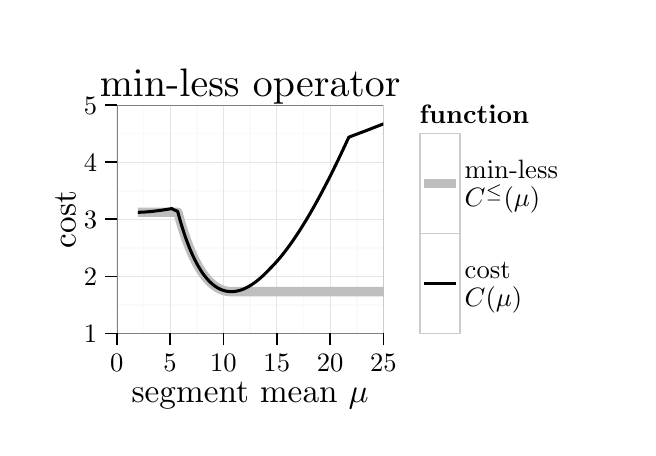
\begin{tikzpicture}[x=1pt,y=1pt]
\definecolor{fillColor}{RGB}{255,255,255}
\path[use as bounding box,fill=fillColor,fill opacity=0.00] (0,0) rectangle (216.81,144.54);
\begin{scope}
\path[clip] (  0.00,  0.00) rectangle (216.81,144.54);
\definecolor{drawColor}{RGB}{255,255,255}
\definecolor{fillColor}{RGB}{255,255,255}

\path[draw=drawColor,line width= 0.6pt,line join=round,line cap=round,fill=fillColor] (  0.00, -0.00) rectangle (216.81,144.54);
\end{scope}
\begin{scope}
\path[clip] ( 32.22, 34.03) rectangle (128.53,116.55);
\definecolor{fillColor}{RGB}{255,255,255}

\path[fill=fillColor] ( 32.22, 34.03) rectangle (128.53,116.55);
\definecolor{drawColor}{gray}{0.98}

\path[draw=drawColor,line width= 0.6pt,line join=round] ( 32.22, 44.35) --
	(128.53, 44.35);

\path[draw=drawColor,line width= 0.6pt,line join=round] ( 32.22, 64.98) --
	(128.53, 64.98);

\path[draw=drawColor,line width= 0.6pt,line join=round] ( 32.22, 85.61) --
	(128.53, 85.61);

\path[draw=drawColor,line width= 0.6pt,line join=round] ( 32.22,106.24) --
	(128.53,106.24);

\path[draw=drawColor,line width= 0.6pt,line join=round] ( 41.85, 34.03) --
	( 41.85,116.55);

\path[draw=drawColor,line width= 0.6pt,line join=round] ( 61.12, 34.03) --
	( 61.12,116.55);

\path[draw=drawColor,line width= 0.6pt,line join=round] ( 80.38, 34.03) --
	( 80.38,116.55);

\path[draw=drawColor,line width= 0.6pt,line join=round] ( 99.64, 34.03) --
	( 99.64,116.55);

\path[draw=drawColor,line width= 0.6pt,line join=round] (118.90, 34.03) --
	(118.90,116.55);
\definecolor{drawColor}{gray}{0.90}

\path[draw=drawColor,line width= 0.2pt,line join=round] ( 32.22, 34.03) --
	(128.53, 34.03);

\path[draw=drawColor,line width= 0.2pt,line join=round] ( 32.22, 54.66) --
	(128.53, 54.66);

\path[draw=drawColor,line width= 0.2pt,line join=round] ( 32.22, 75.29) --
	(128.53, 75.29);

\path[draw=drawColor,line width= 0.2pt,line join=round] ( 32.22, 95.92) --
	(128.53, 95.92);

\path[draw=drawColor,line width= 0.2pt,line join=round] ( 32.22,116.55) --
	(128.53,116.55);

\path[draw=drawColor,line width= 0.2pt,line join=round] ( 32.22, 34.03) --
	( 32.22,116.55);

\path[draw=drawColor,line width= 0.2pt,line join=round] ( 51.48, 34.03) --
	( 51.48,116.55);

\path[draw=drawColor,line width= 0.2pt,line join=round] ( 70.75, 34.03) --
	( 70.75,116.55);

\path[draw=drawColor,line width= 0.2pt,line join=round] ( 90.01, 34.03) --
	( 90.01,116.55);

\path[draw=drawColor,line width= 0.2pt,line join=round] (109.27, 34.03) --
	(109.27,116.55);

\path[draw=drawColor,line width= 0.2pt,line join=round] (128.53, 34.03) --
	(128.53,116.55);
\definecolor{drawColor}{RGB}{190,190,190}

\path[draw=drawColor,line width= 3.4pt,line join=round] ( 39.81, 77.83) --
	( 39.96, 77.83) --
	( 40.10, 77.83) --
	( 40.25, 77.83) --
	( 40.40, 77.83) --
	( 40.54, 77.83) --
	( 40.69, 77.83) --
	( 40.83, 77.83) --
	( 40.98, 77.83) --
	( 41.13, 77.83) --
	( 41.27, 77.83) --
	( 41.42, 77.83) --
	( 41.56, 77.83) --
	( 41.71, 77.83) --
	( 41.86, 77.83) --
	( 42.00, 77.83) --
	( 42.15, 77.83) --
	( 42.30, 77.83) --
	( 42.44, 77.83) --
	( 42.59, 77.83) --
	( 42.73, 77.83) --
	( 42.88, 77.83) --
	( 43.03, 77.83) --
	( 43.17, 77.83) --
	( 43.32, 77.83) --
	( 43.46, 77.83) --
	( 43.61, 77.83) --
	( 43.76, 77.83) --
	( 43.90, 77.83) --
	( 44.05, 77.83) --
	( 44.20, 77.83) --
	( 44.34, 77.83) --
	( 44.49, 77.83) --
	( 44.63, 77.83) --
	( 44.78, 77.83) --
	( 44.93, 77.83) --
	( 45.07, 77.83) --
	( 45.22, 77.83) --
	( 45.37, 77.83) --
	( 45.51, 77.83) --
	( 45.66, 77.83) --
	( 45.80, 77.83) --
	( 45.95, 77.83) --
	( 46.10, 77.83) --
	( 46.24, 77.83) --
	( 46.39, 77.83) --
	( 46.53, 77.83) --
	( 46.68, 77.83) --
	( 46.83, 77.83) --
	( 46.97, 77.83) --
	( 47.12, 77.83) --
	( 47.27, 77.83) --
	( 47.41, 77.83) --
	( 47.56, 77.83) --
	( 47.70, 77.83) --
	( 47.85, 77.83) --
	( 48.00, 77.83) --
	( 48.14, 77.83) --
	( 48.29, 77.83) --
	( 48.43, 77.83) --
	( 48.58, 77.83) --
	( 48.73, 77.83) --
	( 48.87, 77.83) --
	( 49.02, 77.83) --
	( 49.17, 77.83) --
	( 49.31, 77.83) --
	( 49.46, 77.83) --
	( 49.60, 77.83) --
	( 49.75, 77.83) --
	( 49.90, 77.83) --
	( 50.04, 77.83) --
	( 50.19, 77.83) --
	( 50.33, 77.83) --
	( 50.48, 77.83) --
	( 50.63, 77.83) --
	( 50.77, 77.83) --
	( 50.92, 77.83) --
	( 51.07, 77.83) --
	( 51.21, 77.83) --
	( 51.36, 77.83) --
	( 51.50, 77.83) --
	( 51.65, 77.83) --
	( 51.80, 77.83) --
	( 51.94, 77.83) --
	( 52.09, 77.83) --
	( 52.23, 77.83) --
	( 52.38, 77.83) --
	( 52.53, 77.83) --
	( 52.67, 77.83) --
	( 52.82, 77.83) --
	( 52.97, 77.83) --
	( 53.11, 77.83) --
	( 53.26, 77.83) --
	( 53.40, 77.83) --
	( 53.55, 77.83) --
	( 53.70, 77.83) --
	( 53.84, 77.83) --
	( 53.99, 77.83) --
	( 54.13, 77.83) --
	( 54.28, 77.83) --
	( 54.28, 77.83) --
	( 54.48, 77.11) --
	( 54.67, 76.40) --
	( 54.87, 75.70) --
	( 55.06, 75.02) --
	( 55.25, 74.35) --
	( 55.45, 73.69) --
	( 55.64, 73.05) --
	( 55.84, 72.41) --
	( 56.03, 71.79) --
	( 56.23, 71.18) --
	( 56.42, 70.58) --
	( 56.62, 70.00) --
	( 56.81, 69.42) --
	( 57.01, 68.86) --
	( 57.20, 68.31) --
	( 57.40, 67.77) --
	( 57.59, 67.24) --
	( 57.79, 66.72) --
	( 57.98, 66.20) --
	( 58.18, 65.70) --
	( 58.37, 65.21) --
	( 58.57, 64.73) --
	( 58.76, 64.26) --
	( 58.96, 63.80) --
	( 59.15, 63.35) --
	( 59.35, 62.91) --
	( 59.54, 62.47) --
	( 59.74, 62.05) --
	( 59.93, 61.64) --
	( 60.13, 61.23) --
	( 60.32, 60.83) --
	( 60.52, 60.44) --
	( 60.71, 60.06) --
	( 60.91, 59.69) --
	( 61.10, 59.32) --
	( 61.30, 58.97) --
	( 61.49, 58.62) --
	( 61.69, 58.28) --
	( 61.88, 57.94) --
	( 62.08, 57.62) --
	( 62.27, 57.30) --
	( 62.47, 56.99) --
	( 62.66, 56.69) --
	( 62.86, 56.39) --
	( 63.05, 56.10) --
	( 63.24, 55.82) --
	( 63.44, 55.55) --
	( 63.63, 55.28) --
	( 63.83, 55.02) --
	( 64.02, 54.77) --
	( 64.22, 54.52) --
	( 64.41, 54.28) --
	( 64.61, 54.04) --
	( 64.80, 53.81) --
	( 65.00, 53.59) --
	( 65.19, 53.38) --
	( 65.39, 53.17) --
	( 65.58, 52.97) --
	( 65.78, 52.77) --
	( 65.97, 52.58) --
	( 66.17, 52.39) --
	( 66.36, 52.21) --
	( 66.56, 52.04) --
	( 66.75, 51.87) --
	( 66.95, 51.71) --
	( 67.14, 51.55) --
	( 67.34, 51.40) --
	( 67.53, 51.26) --
	( 67.73, 51.12) --
	( 67.92, 50.98) --
	( 68.12, 50.85) --
	( 68.31, 50.73) --
	( 68.51, 50.61) --
	( 68.70, 50.50) --
	( 68.90, 50.39) --
	( 69.09, 50.28) --
	( 69.29, 50.18) --
	( 69.48, 50.09) --
	( 69.68, 50.00) --
	( 69.87, 49.92) --
	( 70.07, 49.84) --
	( 70.26, 49.76) --
	( 70.46, 49.69) --
	( 70.65, 49.62) --
	( 70.85, 49.56) --
	( 71.04, 49.51) --
	( 71.23, 49.45) --
	( 71.43, 49.41) --
	( 71.62, 49.36) --
	( 71.82, 49.32) --
	( 72.01, 49.29) --
	( 72.21, 49.26) --
	( 72.40, 49.23) --
	( 72.60, 49.21) --
	( 72.79, 49.19) --
	( 72.99, 49.18) --
	( 73.18, 49.17) --
	( 73.38, 49.16) --
	( 73.57, 49.16) --
	( 73.57, 49.16) --
	( 81.49, 49.16) --
	( 89.41, 49.16) --
	( 97.33, 49.16) --
	(105.25, 49.16) --
	(113.17, 49.16) --
	(121.09, 49.16) --
	(129.01, 49.16) --
	(136.93, 49.16) --
	(144.85, 49.16) --
	(152.77, 49.16) --
	(160.69, 49.16) --
	(168.60, 49.16) --
	(176.52, 49.16) --
	(184.44, 49.16) --
	(192.36, 49.16) --
	(200.28, 49.16) --
	(208.20, 49.16) --
	(216.12, 49.16) --
	(216.81, 49.16);
\definecolor{drawColor}{RGB}{0,0,0}

\path[draw=drawColor,line width= 1.1pt,line join=round] ( 39.81, 77.83) --
	( 39.94, 77.83) --
	( 40.06, 77.83) --
	( 40.18, 77.83) --
	( 40.31, 77.84) --
	( 40.43, 77.84) --
	( 40.55, 77.84) --
	( 40.68, 77.84) --
	( 40.80, 77.85) --
	( 40.93, 77.85) --
	( 41.05, 77.86) --
	( 41.17, 77.86) --
	( 41.30, 77.87) --
	( 41.42, 77.87) --
	( 41.55, 77.88) --
	( 41.67, 77.88) --
	( 41.79, 77.89) --
	( 41.92, 77.90) --
	( 42.04, 77.90) --
	( 42.17, 77.91) --
	( 42.29, 77.92) --
	( 42.41, 77.93) --
	( 42.54, 77.94) --
	( 42.66, 77.95) --
	( 42.79, 77.96) --
	( 42.91, 77.96) --
	( 43.03, 77.97) --
	( 43.16, 77.98) --
	( 43.28, 77.99) --
	( 43.41, 78.01) --
	( 43.53, 78.02) --
	( 43.65, 78.03) --
	( 43.78, 78.04) --
	( 43.90, 78.05) --
	( 44.03, 78.06) --
	( 44.15, 78.07) --
	( 44.27, 78.09) --
	( 44.40, 78.10) --
	( 44.52, 78.11) --
	( 44.65, 78.12) --
	( 44.77, 78.14) --
	( 44.89, 78.15) --
	( 45.02, 78.16) --
	( 45.14, 78.18) --
	( 45.26, 78.19) --
	( 45.39, 78.20) --
	( 45.51, 78.22) --
	( 45.64, 78.23) --
	( 45.76, 78.25) --
	( 45.88, 78.26) --
	( 46.01, 78.28) --
	( 46.13, 78.29) --
	( 46.26, 78.31) --
	( 46.38, 78.32) --
	( 46.50, 78.34) --
	( 46.63, 78.35) --
	( 46.75, 78.37) --
	( 46.88, 78.39) --
	( 47.00, 78.40) --
	( 47.12, 78.42) --
	( 47.25, 78.43) --
	( 47.37, 78.45) --
	( 47.50, 78.47) --
	( 47.62, 78.48) --
	( 47.74, 78.50) --
	( 47.87, 78.52) --
	( 47.99, 78.54) --
	( 48.12, 78.55) --
	( 48.24, 78.57) --
	( 48.36, 78.59) --
	( 48.49, 78.60) --
	( 48.61, 78.62) --
	( 48.74, 78.64) --
	( 48.86, 78.66) --
	( 48.98, 78.68) --
	( 49.11, 78.69) --
	( 49.23, 78.71) --
	( 49.36, 78.73) --
	( 49.48, 78.75) --
	( 49.60, 78.77) --
	( 49.73, 78.79) --
	( 49.85, 78.81) --
	( 49.98, 78.83) --
	( 50.10, 78.84) --
	( 50.22, 78.86) --
	( 50.35, 78.88) --
	( 50.47, 78.90) --
	( 50.59, 78.92) --
	( 50.72, 78.94) --
	( 50.84, 78.96) --
	( 50.97, 78.98) --
	( 51.09, 79.00) --
	( 51.21, 79.02) --
	( 51.34, 79.04) --
	( 51.46, 79.06) --
	( 51.59, 79.08) --
	( 51.71, 79.10) --
	( 51.83, 79.12) --
	( 51.96, 79.14) --
	( 52.08, 79.16) --
	( 52.08, 79.16) --
	( 52.10, 79.15) --
	( 52.12, 79.14) --
	( 52.15, 79.13) --
	( 52.17, 79.12) --
	( 52.19, 79.10) --
	( 52.21, 79.09) --
	( 52.23, 79.08) --
	( 52.25, 79.07) --
	( 52.27, 79.06) --
	( 52.30, 79.05) --
	( 52.32, 79.04) --
	( 52.34, 79.02) --
	( 52.36, 79.01) --
	( 52.38, 79.00) --
	( 52.40, 78.99) --
	( 52.42, 78.98) --
	( 52.44, 78.97) --
	( 52.47, 78.96) --
	( 52.49, 78.95) --
	( 52.51, 78.93) --
	( 52.53, 78.92) --
	( 52.55, 78.91) --
	( 52.57, 78.90) --
	( 52.59, 78.89) --
	( 52.61, 78.88) --
	( 52.64, 78.87) --
	( 52.66, 78.86) --
	( 52.68, 78.85) --
	( 52.70, 78.84) --
	( 52.72, 78.83) --
	( 52.74, 78.82) --
	( 52.76, 78.81) --
	( 52.78, 78.80) --
	( 52.81, 78.78) --
	( 52.83, 78.77) --
	( 52.85, 78.76) --
	( 52.87, 78.75) --
	( 52.89, 78.74) --
	( 52.91, 78.73) --
	( 52.93, 78.72) --
	( 52.96, 78.71) --
	( 52.98, 78.70) --
	( 53.00, 78.69) --
	( 53.02, 78.68) --
	( 53.04, 78.67) --
	( 53.06, 78.66) --
	( 53.08, 78.65) --
	( 53.10, 78.64) --
	( 53.13, 78.63) --
	( 53.15, 78.62) --
	( 53.17, 78.61) --
	( 53.19, 78.60) --
	( 53.21, 78.59) --
	( 53.23, 78.58) --
	( 53.25, 78.57) --
	( 53.27, 78.56) --
	( 53.30, 78.55) --
	( 53.32, 78.54) --
	( 53.34, 78.53) --
	( 53.36, 78.52) --
	( 53.38, 78.51) --
	( 53.40, 78.50) --
	( 53.42, 78.49) --
	( 53.44, 78.48) --
	( 53.47, 78.48) --
	( 53.49, 78.47) --
	( 53.51, 78.46) --
	( 53.53, 78.45) --
	( 53.55, 78.44) --
	( 53.57, 78.43) --
	( 53.59, 78.42) --
	( 53.62, 78.41) --
	( 53.64, 78.40) --
	( 53.66, 78.39) --
	( 53.68, 78.38) --
	( 53.70, 78.37) --
	( 53.72, 78.36) --
	( 53.74, 78.36) --
	( 53.76, 78.35) --
	( 53.79, 78.34) --
	( 53.81, 78.33) --
	( 53.83, 78.32) --
	( 53.85, 78.31) --
	( 53.87, 78.30) --
	( 53.89, 78.29) --
	( 53.91, 78.28) --
	( 53.93, 78.27) --
	( 53.96, 78.27) --
	( 53.98, 78.26) --
	( 54.00, 78.25) --
	( 54.02, 78.24) --
	( 54.04, 78.23) --
	( 54.06, 78.22) --
	( 54.08, 78.21) --
	( 54.10, 78.21) --
	( 54.13, 78.20) --
	( 54.15, 78.19) --
	( 54.17, 78.18) --
	( 54.19, 78.17) --
	( 54.19, 78.17) --
	( 54.53, 76.92) --
	( 54.87, 75.70) --
	( 55.20, 74.52) --
	( 55.54, 73.38) --
	( 55.88, 72.28) --
	( 56.22, 71.22) --
	( 56.56, 70.19) --
	( 56.89, 69.19) --
	( 57.23, 68.23) --
	( 57.57, 67.30) --
	( 57.91, 66.40) --
	( 58.24, 65.54) --
	( 58.58, 64.70) --
	( 58.92, 63.89) --
	( 59.26, 63.11) --
	( 59.60, 62.36) --
	( 59.93, 61.63) --
	( 60.27, 60.93) --
	( 60.61, 60.26) --
	( 60.95, 59.61) --
	( 61.29, 58.98) --
	( 61.62, 58.38) --
	( 61.96, 57.81) --
	( 62.30, 57.25) --
	( 62.64, 56.72) --
	( 62.98, 56.21) --
	( 63.31, 55.72) --
	( 63.65, 55.26) --
	( 63.99, 54.81) --
	( 64.33, 54.38) --
	( 64.67, 53.98) --
	( 65.00, 53.59) --
	( 65.34, 53.22) --
	( 65.68, 52.87) --
	( 66.02, 52.54) --
	( 66.35, 52.22) --
	( 66.69, 51.92) --
	( 67.03, 51.64) --
	( 67.37, 51.38) --
	( 67.71, 51.13) --
	( 68.04, 50.90) --
	( 68.38, 50.68) --
	( 68.72, 50.48) --
	( 69.06, 50.30) --
	( 69.40, 50.13) --
	( 69.73, 49.97) --
	( 70.07, 49.83) --
	( 70.41, 49.71) --
	( 70.75, 49.59) --
	( 71.09, 49.49) --
	( 71.42, 49.41) --
	( 71.76, 49.34) --
	( 72.10, 49.28) --
	( 72.44, 49.23) --
	( 72.78, 49.19) --
	( 73.11, 49.17) --
	( 73.45, 49.16) --
	( 73.79, 49.16) --
	( 74.13, 49.18) --
	( 74.46, 49.20) --
	( 74.80, 49.24) --
	( 75.14, 49.28) --
	( 75.48, 49.34) --
	( 75.82, 49.41) --
	( 76.15, 49.49) --
	( 76.49, 49.58) --
	( 76.83, 49.68) --
	( 77.17, 49.79) --
	( 77.51, 49.91) --
	( 77.84, 50.04) --
	( 78.18, 50.18) --
	( 78.52, 50.33) --
	( 78.86, 50.49) --
	( 79.20, 50.66) --
	( 79.53, 50.84) --
	( 79.87, 51.03) --
	( 80.21, 51.22) --
	( 80.55, 51.43) --
	( 80.89, 51.64) --
	( 81.22, 51.86) --
	( 81.56, 52.09) --
	( 81.90, 52.33) --
	( 82.24, 52.58) --
	( 82.57, 52.83) --
	( 82.91, 53.10) --
	( 83.25, 53.37) --
	( 83.59, 53.64) --
	( 83.93, 53.93) --
	( 84.26, 54.22) --
	( 84.60, 54.53) --
	( 84.94, 54.83) --
	( 85.28, 55.15) --
	( 85.62, 55.47) --
	( 85.95, 55.80) --
	( 86.29, 56.14) --
	( 86.63, 56.48) --
	( 86.97, 56.83) --
	( 87.31, 57.19) --
	( 87.64, 57.56) --
	( 87.64, 57.56) --
	( 87.93, 57.84) --
	( 88.22, 58.13) --
	( 88.50, 58.43) --
	( 88.79, 58.73) --
	( 89.08, 59.03) --
	( 89.36, 59.34) --
	( 89.65, 59.66) --
	( 89.94, 59.98) --
	( 90.22, 60.30) --
	( 90.51, 60.63) --
	( 90.80, 60.96) --
	( 91.09, 61.30) --
	( 91.37, 61.65) --
	( 91.66, 62.00) --
	( 91.95, 62.35) --
	( 92.23, 62.71) --
	( 92.52, 63.07) --
	( 92.81, 63.44) --
	( 93.09, 63.81) --
	( 93.38, 64.18) --
	( 93.67, 64.56) --
	( 93.95, 64.95) --
	( 94.24, 65.34) --
	( 94.53, 65.73) --
	( 94.81, 66.13) --
	( 95.10, 66.53) --
	( 95.39, 66.93) --
	( 95.67, 67.34) --
	( 95.96, 67.76) --
	( 96.25, 68.17) --
	( 96.53, 68.59) --
	( 96.82, 69.02) --
	( 97.11, 69.45) --
	( 97.39, 69.88) --
	( 97.68, 70.32) --
	( 97.97, 70.76) --
	( 98.25, 71.20) --
	( 98.54, 71.65) --
	( 98.83, 72.10) --
	( 99.11, 72.56) --
	( 99.40, 73.02) --
	( 99.69, 73.48) --
	( 99.98, 73.95) --
	(100.26, 74.42) --
	(100.55, 74.89) --
	(100.84, 75.37) --
	(101.12, 75.85) --
	(101.41, 76.33) --
	(101.70, 76.82) --
	(101.98, 77.31) --
	(102.27, 77.80) --
	(102.56, 78.30) --
	(102.84, 78.80) --
	(103.13, 79.31) --
	(103.42, 79.81) --
	(103.70, 80.32) --
	(103.99, 80.84) --
	(104.28, 81.35) --
	(104.56, 81.87) --
	(104.85, 82.39) --
	(105.14, 82.92) --
	(105.42, 83.45) --
	(105.71, 83.98) --
	(106.00, 84.52) --
	(106.28, 85.05) --
	(106.57, 85.60) --
	(106.86, 86.14) --
	(107.14, 86.69) --
	(107.43, 87.24) --
	(107.72, 87.79) --
	(108.01, 88.34) --
	(108.29, 88.90) --
	(108.58, 89.46) --
	(108.87, 90.03) --
	(109.15, 90.59) --
	(109.44, 91.16) --
	(109.73, 91.73) --
	(110.01, 92.31) --
	(110.30, 92.89) --
	(110.59, 93.47) --
	(110.87, 94.05) --
	(111.16, 94.64) --
	(111.45, 95.22) --
	(111.73, 95.81) --
	(112.02, 96.41) --
	(112.31, 97.00) --
	(112.59, 97.60) --
	(112.88, 98.20) --
	(113.17, 98.81) --
	(113.45, 99.41) --
	(113.74,100.02) --
	(114.03,100.63) --
	(114.31,101.24) --
	(114.60,101.86) --
	(114.89,102.48) --
	(115.17,103.10) --
	(115.46,103.72) --
	(115.75,104.34) --
	(116.04,104.97) --
	(116.04,104.97) --
	(123.53,107.81) --
	(131.02,110.74) --
	(138.51,113.74) --
	(146.00,116.82) --
	(153.49,119.96) --
	(160.98,123.14) --
	(168.47,126.38) --
	(175.96,129.66) --
	(183.45,132.97) --
	(190.94,136.32) --
	(198.43,139.69) --
	(205.92,143.10) --
	(209.06,144.54);
\definecolor{drawColor}{gray}{0.50}

\path[draw=drawColor,line width= 0.6pt,line join=round,line cap=round] ( 32.22, 34.03) rectangle (128.53,116.55);
\end{scope}
\begin{scope}
\path[clip] (  0.00,  0.00) rectangle (216.81,144.54);
\definecolor{drawColor}{RGB}{0,0,0}

\node[text=drawColor,anchor=base east,inner sep=0pt, outer sep=0pt, scale=  0.96] at ( 25.11, 30.73) {1};

\node[text=drawColor,anchor=base east,inner sep=0pt, outer sep=0pt, scale=  0.96] at ( 25.11, 51.36) {2};

\node[text=drawColor,anchor=base east,inner sep=0pt, outer sep=0pt, scale=  0.96] at ( 25.11, 71.99) {3};

\node[text=drawColor,anchor=base east,inner sep=0pt, outer sep=0pt, scale=  0.96] at ( 25.11, 92.62) {4};

\node[text=drawColor,anchor=base east,inner sep=0pt, outer sep=0pt, scale=  0.96] at ( 25.11,113.25) {5};
\end{scope}
\begin{scope}
\path[clip] (  0.00,  0.00) rectangle (216.81,144.54);
\definecolor{drawColor}{RGB}{0,0,0}

\path[draw=drawColor,line width= 0.6pt,line join=round] ( 27.95, 34.03) --
	( 32.22, 34.03);

\path[draw=drawColor,line width= 0.6pt,line join=round] ( 27.95, 54.66) --
	( 32.22, 54.66);

\path[draw=drawColor,line width= 0.6pt,line join=round] ( 27.95, 75.29) --
	( 32.22, 75.29);

\path[draw=drawColor,line width= 0.6pt,line join=round] ( 27.95, 95.92) --
	( 32.22, 95.92);

\path[draw=drawColor,line width= 0.6pt,line join=round] ( 27.95,116.55) --
	( 32.22,116.55);
\end{scope}
\begin{scope}
\path[clip] (  0.00,  0.00) rectangle (216.81,144.54);
\definecolor{drawColor}{RGB}{0,0,0}

\path[draw=drawColor,line width= 0.6pt,line join=round] ( 32.22, 29.77) --
	( 32.22, 34.03);

\path[draw=drawColor,line width= 0.6pt,line join=round] ( 51.48, 29.77) --
	( 51.48, 34.03);

\path[draw=drawColor,line width= 0.6pt,line join=round] ( 70.75, 29.77) --
	( 70.75, 34.03);

\path[draw=drawColor,line width= 0.6pt,line join=round] ( 90.01, 29.77) --
	( 90.01, 34.03);

\path[draw=drawColor,line width= 0.6pt,line join=round] (109.27, 29.77) --
	(109.27, 34.03);

\path[draw=drawColor,line width= 0.6pt,line join=round] (128.53, 29.77) --
	(128.53, 34.03);
\end{scope}
\begin{scope}
\path[clip] (  0.00,  0.00) rectangle (216.81,144.54);
\definecolor{drawColor}{RGB}{0,0,0}

\node[text=drawColor,anchor=base,inner sep=0pt, outer sep=0pt, scale=  0.96] at ( 32.22, 20.31) {0};

\node[text=drawColor,anchor=base,inner sep=0pt, outer sep=0pt, scale=  0.96] at ( 51.48, 20.31) {5};

\node[text=drawColor,anchor=base,inner sep=0pt, outer sep=0pt, scale=  0.96] at ( 70.75, 20.31) {10};

\node[text=drawColor,anchor=base,inner sep=0pt, outer sep=0pt, scale=  0.96] at ( 90.01, 20.31) {15};

\node[text=drawColor,anchor=base,inner sep=0pt, outer sep=0pt, scale=  0.96] at (109.27, 20.31) {20};

\node[text=drawColor,anchor=base,inner sep=0pt, outer sep=0pt, scale=  0.96] at (128.53, 20.31) {25};
\end{scope}
\begin{scope}
\path[clip] (  0.00,  0.00) rectangle (216.81,144.54);
\definecolor{drawColor}{RGB}{0,0,0}

\node[text=drawColor,anchor=base,inner sep=0pt, outer sep=0pt, scale=  1.20] at ( 80.38,  9.03) {segment mean $\mu$};
\end{scope}
\begin{scope}
\path[clip] (  0.00,  0.00) rectangle (216.81,144.54);
\definecolor{drawColor}{RGB}{0,0,0}

\node[text=drawColor,rotate= 90.00,anchor=base,inner sep=0pt, outer sep=0pt, scale=  1.20] at ( 17.30, 75.29) {cost};
\end{scope}
\begin{scope}
\path[clip] (  0.00,  0.00) rectangle (216.81,144.54);
\definecolor{fillColor}{RGB}{255,255,255}

\path[fill=fillColor] (137.40, 29.77) rectangle (195.90,120.82);
\end{scope}
\begin{scope}
\path[clip] (  0.00,  0.00) rectangle (216.81,144.54);
\definecolor{drawColor}{RGB}{0,0,0}

\node[text=drawColor,anchor=base west,inner sep=0pt, outer sep=0pt, scale=  0.96] at (141.67,109.92) {\bfseries function};
\end{scope}
\begin{scope}
\path[clip] (  0.00,  0.00) rectangle (216.81,144.54);
\definecolor{drawColor}{gray}{0.80}
\definecolor{fillColor}{RGB}{255,255,255}

\path[draw=drawColor,line width= 0.6pt,line join=round,line cap=round,fill=fillColor] (141.67, 70.18) rectangle (156.12,106.31);
\end{scope}
\begin{scope}
\path[clip] (  0.00,  0.00) rectangle (216.81,144.54);
\definecolor{drawColor}{RGB}{190,190,190}

\path[draw=drawColor,line width= 3.4pt,line join=round] (143.12, 88.24) -- (154.68, 88.24);
\end{scope}
\begin{scope}
\path[clip] (  0.00,  0.00) rectangle (216.81,144.54);
\definecolor{drawColor}{gray}{0.80}
\definecolor{fillColor}{RGB}{255,255,255}

\path[draw=drawColor,line width= 0.6pt,line join=round,line cap=round,fill=fillColor] (141.67, 34.04) rectangle (156.12, 70.18);
\end{scope}
\begin{scope}
\path[clip] (  0.00,  0.00) rectangle (216.81,144.54);
\definecolor{drawColor}{RGB}{0,0,0}

\path[draw=drawColor,line width= 1.1pt,line join=round] (143.12, 52.11) -- (154.68, 52.11);
\end{scope}
\begin{scope}
\path[clip] (  0.00,  0.00) rectangle (216.81,144.54);
\definecolor{drawColor}{RGB}{0,0,0}

\node[text=drawColor,anchor=base west,inner sep=0pt, outer sep=0pt, scale=  0.96] at (157.93, 90.12) {min-less};

\node[text=drawColor,anchor=base west,inner sep=0pt, outer sep=0pt, scale=  0.96] at (157.93, 79.75) {$C^{\leq}(\mu)$};
\end{scope}
\begin{scope}
\path[clip] (  0.00,  0.00) rectangle (216.81,144.54);
\definecolor{drawColor}{RGB}{0,0,0}

\node[text=drawColor,anchor=base west,inner sep=0pt, outer sep=0pt, scale=  0.96] at (157.93, 53.99) {cost};

\node[text=drawColor,anchor=base west,inner sep=0pt, outer sep=0pt, scale=  0.96] at (157.93, 43.62) {$C(\mu)$};
\end{scope}
\begin{scope}
\path[clip] (  0.00,  0.00) rectangle (216.81,144.54);
\definecolor{drawColor}{RGB}{0,0,0}

\node[text=drawColor,anchor=base,inner sep=0pt, outer sep=0pt, scale=  1.44] at ( 80.38,119.57) {min-less operator};
\end{scope}
\end{tikzpicture}

    \end{center}
  }
  \caption{\label{fig:min-operators} Min-less and min-more
    functions need to be computed exactly and represented as piecewise
    functions.}
\end{figure}

The next step is to compute the minimum cost in 2 segments up to data
point 3, for which there is a choice of two change-points.
\begin{equation*}
  C_{2,3}(\mu) = \min
  \begin{cases}
    C_{2,2}(\mu)+\gamma_3(\mu), \\
    C_{1,2}^{\leq}(\mu)+\gamma_3(\mu)
  \end{cases}
\end{equation*}
We have already computed an exact representation of the $C_{2,2}$
term, which is the cost a change after the first data point. Now we
need to compare it with the $C_{1,2}^{\leq}$ term, which is the cost
of a change after the second data point. This is a crucial step in
which the \texttt{MinEnvelope} sub-routine computes an exact
representation of the minimum of these two functions.

The updates continue for every data point $b\in\{3, ..., B\}$
\begin{equation*}
  C_{2,b}(\mu) = \min
  \begin{cases}
    C_{2,b-1}(\mu) + \gamma_b(\mu),\\
    C_{1,b-1}^{\leq}(\mu) + \gamma_b(\mu).
  \end{cases}
\end{equation*}

For the third segment we first compute the minimum cost up to data point 3
\begin{equation*}
  C_{3,3}(\mu) = C_{2,2}^{\geq}(\mu) + \gamma_3(\mu),
\end{equation*}
where the more-min operator $f^\geq$ is defined analogously. The
update formula for the minimum cost up to data point
$b\in\{4, ..., B\}$ is
\begin{equation*}
  C_{3,b}(\mu) = \min
  \begin{cases}
    C_{3,b-1}^{\geq}(\mu)+\gamma_b(\mu),\\
    C_{2,b-1}^{\geq}(\mu)+\gamma_b(\mu)
  \end{cases}
\end{equation*}
In general for $s$ segments, we use
\begin{equation}
  C_{s,s}(\mu) = C_{s-1,s-1}^{*}(\mu) + \gamma_s(\mu),
\end{equation}
and for $b\in\{s+1, ..., B\}$
\begin{equation}
  C_{s,b}(\mu) = \min
  \begin{cases}
    C_{s,b-1}^{*}(\mu)+\gamma_b(\mu),\\
    C_{s-1,b-1}^{*}(\mu)+\gamma_b(\mu),
  \end{cases}
\end{equation}
where * means less-min for even-numbered segments $s$, and more-min
for odd-numbered segments.

\subsection{Optimal Partitioning}

\section{Figures}

\subsection{Simple data set analysis}

In this section we analyze the simple data
$\mathbf z = \left[\begin{array}{cccc} 1 & 10 & 14 & 13
\end{array}\right]\in\ZZ_+^4
$. For $s=3$ segments there are only 3 possible segmentations:
$[1][10][14, 13]$, $[1][10, 14][13]$ and $[1, 10][14][13]$. If we use
max-likelihood estimates for each segment mean, then only the last
segmentation obeys the \ref{PenPeakSeg} model constraints. However the
constrained Dynamic Programming Algorithm of \citet{PeakSeg} does not
recover it. However this last segmentation is more costly than a
simpler segmentation with a single change after the first data point
(see figure below).

\includegraphics[width=\textwidth]{figure-constrained-PDPA-normal-grid}

The figure above plots the cost of a segmentation in two segments, up
to data point 3. There are two possible change-points: after 1 [1][10
14], and after 2 [1 10][14]. The minimum cost of a change after 2 is
40.5, but the other change is less costly for those mean values (5.5,
14). Thus it is clear that although the segmentation [1 10][14][13] is
feasible for the PeakSeg problem, it is clearly not optimal.

\subsection{Unconstrained PDPA and FPOP}

In the figures below I took the R implementation of PDPA and FPOP from
the FPOP paper, and I ran both on this simple data set. The plot shows
the functions and intervals at each time step. The first column shows
the model ofthe cost before adding a new data point, the second column
shows after adding a new data point but before pruning, and the third
column shows after pruning.

\includegraphics[width=\textwidth]{figure-unconstrained-FPOP-normal}

\includegraphics[width=\textwidth]{figure-unconstrained-PDPA-normal}

The figure above shows the same results for the unconstrained PDPA.

\subsection{Results with and without strict inequalities}

\includegraphics[width=\textwidth]{figure-constrained-PDPA-normal-panels-pruning}

The figure above compares the results of the two different cost models
(with and without strict inequalities). Note that for strict
inequalities it is a bit more complicated to compute the less-min
operator. In fact the minimum $\mu^*$ may be undefined, in which case
we set $f^{<}(\mu)=\infty$ (infinite cost intervals are not
stored). Otherwise if $\mu^*$ is achieved somewhere in the domain of
$f$ we use
\begin{equation*}
  f^{<}(\mu) = \min_{x<\mu}f(x) = 
  \begin{cases}
    f(\mu^*) & \text{ if } \mu > \mu^*,\\
    \infty & \text{ otherwise.}
  \end{cases}
\end{equation*}


\includegraphics[width=\textwidth]{figure-constrained-PDPA-normal-panels}

\section{Timings}

TODO: plot the number of intervals over time.

TODO: show that the time complexity is empirically linear in the
number of data points.

\section{Comparison with two-state HMM}

TODO: first run two-state HMM, which will assign a certain number of
peaks. Compute the Poisson loss for that model, and compare it to the
optimal Poisson loss recovered by the PDPA.

\includegraphics[width=\textwidth]{figure-NA-timings}

\bibliographystyle{abbrvnat}
\bibliography{refs}

\end{document}

